% ============================================================
%  midsub.tex -- EVS Project #19 Mid-Evaluation
%  Compound Heat-Drought Stress over India
%
%  Compile with:   pdflatex midsub
%                  bibtex   midsub
%                  pdflatex midsub
%                  pdflatex midsub
%
%  Every number on these slides comes from midSub/results/*.csv (or the
%  printed output of scripts/02-06). See slides/NUMBERS.md for the
%  claim -> source-file map.
% ============================================================
\documentclass[12pt,aspectratio=169]{beamer}

\usetheme{Madrid}
\usecolortheme{seahorse}

\usepackage[T1]{fontenc}
\usepackage[utf8]{inputenc}
\usepackage{tikz}
\usetikzlibrary{positioning, arrows.meta, shapes.geometric}
\usepackage{booktabs}
\usepackage{graphicx}
\usepackage{multirow}

\usepackage{natbib}
\bibliographystyle{unsrtnat}

% Figures come from ../figures/ (written by scripts 02-06). Missing figures
% show a labelled placeholder box so the deck always compiles.
\newcommand{\FigPath}[1]{../figures/#1.png}
\newcommand{\FigureOrPlaceholder}[3]{%
  % #1 = figure stem, #2 = max width, #3 = placeholder caption
  \IfFileExists{\FigPath{#1}}{%
    \includegraphics[width=#2,height=0.68\textheight,keepaspectratio]{\FigPath{#1}}%
  }{%
    \begin{tikzpicture}
      \node[draw, dashed, minimum width=#2, minimum height=0.5\textheight,
            align=center, font=\small\itshape] {#3\\[4pt]\texttt{\detokenize{figures/#1.png}}};
    \end{tikzpicture}%
  }%
}

\title[Compound Heat-Drought Stress]{Compound Heat--Drought Stress over India}
\subtitle{Mid-Evaluation: EVS Project \#19}
\author[Deshmukh et al.]{
  Arnav Deshmukh \and Ayush Brajesh Roy \and Saksham Chitkara \and
  Gracy Garg \and Rudra Choudhary
}
\institute{IIIT Hyderabad}
\date{\today}

\begin{document}

% ---------------------------------------------------------------
\frame{\titlepage}

% ---------------------------------------------------------------
\begin{frame}{Problem Statement}
  \small
  \textbf{Assigned question:} Does simultaneous heat and drought produce
  greater ecosystem stress than either disturbance alone -- and are ecosystems
  experiencing stronger combined impacts?

  \vspace{6pt}
  \begin{itemize}
    \item Two parts: (i) is compound stress worse than heat-only or
      drought-only, and is it worse than their \emph{sum}? (ii) are compound
      conditions becoming more common?
    \item Much of the literature analyses individual compound events (e.g.\
      Europe 2003, \citealp{ciais2005}); fewer studies compare compound,
      heat-only and drought-only conditions against one common baseline
      (\citealp{vonbuttlar2018} is one that does, using flux towers).
    \item India is now being studied: India-wide compound vs single-stressor
      NDVI response \citep{meena2026}; Peninsular forest GPP
      \citep{sen2026}; satellite vegetation response to compound events
      \citep{malik2025}.
    \item Our approach: all of India, 0.25\textdegree{} monthly; vegetation
      2001--2022, climate 1991--2024.
  \end{itemize}
\end{frame}

% ---------------------------------------------------------------
\begin{frame}{From Literature Gaps to Hypotheses}
  \scriptsize
  \renewcommand{\arraystretch}{0.95}
  \begin{tabular}{@{}p{0.27\linewidth}p{0.33\linewidth}p{0.34\linewidth}@{}}
    \toprule
    \textbf{Gap / question} & \textbf{Hypothesis} & \textbf{Test} \\
    \midrule
    Few clean compound-vs-single comparisons &
      H1: GPP/NDVI lower in compound months than in hot-only or dry-only months &
      Category means; joint year-block bootstrap 95\% CIs \\
    &
      H2: the effect is synergistic (worse than the sum) &
      Amplification index with 95\% CI; response surface \\
    Recovery: studies disagree \citep{yao2024,huang2025,feng2026} &
      H3: compound events recover more slowly than droughts &
      Kaplan--Meier, log-rank, severity-matched comparison \\
    India under-studied &
      H4: response differs by land cover and region &
      Same tests per stratum; Peninsular vs North difference \\
    "Stronger impacts" over time? &
      H5: compound conditions are becoming more frequent &
      Sen's slope + Mann--Kendall, 1991--2024 \\
    Definitions vary between studies &
      Results should not hinge on the drought index &
      Repeat H1/H2 with SPI-3 instead of SPEI-3 \\
    \bottomrule
  \end{tabular}
\end{frame}

% ---------------------------------------------------------------
\begin{frame}{Positioning: What Is (and Isn't) New Here}
  \scriptsize
  \begin{columns}[T]
    \column{0.5\linewidth}
    \textbf{Already done by others}
    \begin{itemize}
      \item Compound vs heat-only vs drought-only comparisons: flux towers
        \citep{vonbuttlar2018}, model scenarios \citep{tschumi2023}.
      \item India-wide NDVI response to compound dry--hot extremes, with
        amplification metrics (copula-based probabilities)
        \citep{meena2026}.
      \item Compound hot--dry GPP loss in Peninsular Indian forests
        (MOD17A2H) \citep{sen2026}.
      \item Recovery after compound vs drought events, globally, with
        conflicting answers \citep{yao2024,huang2025,feng2026}.
      \item Rising compound drought--heatwave frequency in India from
        1951 onwards \citep{sharma2017,bhattacharjee2026}.
    \end{itemize}
    \column{0.5\linewidth}
    \textbf{What this project adds}
    \begin{itemize}
      \item An India-wide recovery-time comparison of compound,
        drought-only and heat-only events, matched on drought severity.
        We found no India-specific study of this.
      \item A direct additivity test on \emph{mean} anomalies, with 95\% CIs,
        on both GPP and NDVI, by land cover and region.
      \item A check that conclusions depend on the drought index (SPEI-3 vs
        SPI-3).
      \item A product-consistency finding: MOD17 GPP and NDVI disagree for
        forests.
    \end{itemize}
    \vspace{4pt}
    \textit{Honest framing: a regional synthesis and replication with
    these extensions, not a first-of-its-kind study.}
  \end{columns}
\end{frame}

% ---------------------------------------------------------------
\begin{frame}{Study Area}
  \centering
  \FigureOrPlaceholder{study_area_landcover}{0.55\linewidth}
    {Dominant land cover + Peninsular cutoff (22\textdegree N)}

  \footnotesize Analysis uses only 0.25\textdegree{} cells $\ge$50\% inside
  India (4,481 cells; 4,160 are vegetated and seasonally active).
  Peninsular = cells south of 22\textdegree N. Boundaries from USDOS LSIB
  (illustrative, not authoritative).
\end{frame}

% ---------------------------------------------------------------
\begin{frame}{Data}
  \scriptsize
  \renewcommand{\arraystretch}{0.85}
  \setlength{\tabcolsep}{4pt}
  \begin{tabular}{@{}p{0.2\linewidth}p{0.3\linewidth}p{0.12\linewidth}p{0.3\linewidth}@{}}
    \toprule
    \textbf{Dataset} & \textbf{Variables} & \textbf{Period} & \textbf{Role} \\
    \midrule
    ERA5-Land \citep{munozsabater2021} & daily Tmax (monthly mean), soil moisture 0--100 cm, VPD & 1991--2024 &
      Heat definition; mechanism \\
    CHIRPS v2 \citep{funk2015} & Precipitation & 1991--2024 &
      SPI-3 (temperature-free drought index) \\
    SPEI v2.11 \citep{vicenteserrano2010} & SPEI-3 & 1991--2024 &
      Primary drought definition \\
    MODIS MOD17A2H v006 \citep{running2015,running2004} & GPP & 2001--2022 &
      Primary response \\
    MODIS MOD13A3 v061 \citep{didan2021} & NDVI (QA-masked) & 2001--2022 &
      Second response (greenness) \\
    ESA WorldCover v200 \citep{zanaga2022} & Land-cover fractions & 2021 &
      Strata; vegetation mask \\
    \bottomrule
  \end{tabular}

  \vspace{4pt}
  \tiny All aggregated server-side in Google Earth Engine \citep{gorelick2017}
  to 0.25\textdegree{} (pyramid-based averaging, i.e.\ approximate cell means).
  GPP and NDVI both come from MODIS Terra, so they are two products of one
  sensor, not independent sensors. NDVI cell-months whose mean QA flag is
  cloudy/snow are dropped (14.6\% of active cell-months).
\end{frame}

% ---------------------------------------------------------------
\begin{frame}{Pipeline}
  \centering
  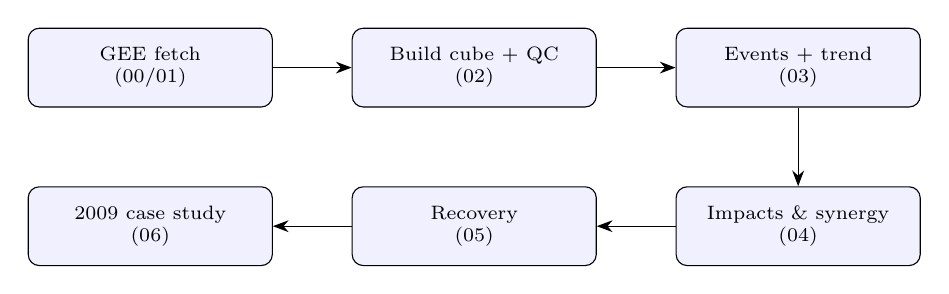
\begin{tikzpicture}[
      node distance=10mm,
      box/.style={draw, rounded corners, align=center, minimum width=3.1cm,
                  minimum height=1cm, font=\scriptsize, fill=blue!6},
      arr/.style={-{Stealth[length=2mm]}}
    ]
    \node[box] (fetch)   {GEE fetch \\ (00/01)};
    \node[box, right=of fetch] (cube)   {Build cube + QC \\ (02)};
    \node[box, right=of cube] (events)  {Events + trend \\ (03)};
    \node[box, below=of events] (impacts) {Impacts \& synergy \\ (04)};
    \node[box, left=of impacts] (recov) {Recovery \\ (05)};
    \node[box, left=of recov] (cases) {2009 case study \\ (06)};
    \draw[arr] (fetch) -- (cube);
    \draw[arr] (cube) -- (events);
    \draw[arr] (events) -- (impacts);
    \draw[arr] (impacts) -- (recov);
    \draw[arr] (recov) -- (cases);
  \end{tikzpicture}

  \vspace{10pt}
  \footnotesize Scripts 02--06 run from cached data only. 64 automated tests
  check the index maths, event logic, statistics and the full pipeline on
  synthetic data.
\end{frame}

% ---------------------------------------------------------------
\begin{frame}{Stress Definitions}
  \begin{columns}
    \column{0.44\linewidth}
    \textbf{Per cell-month:}
    \begin{center}
    \small
    \setlength{\tabcolsep}{3pt}
    \renewcommand{\arraystretch}{1.3}
    \begin{tabular}{cc|c|c}
      & & \multicolumn{2}{c}{SPEI-3} \\
      & & $> -1$ & $\le -1$ \\
      \hline
      \multirow{2}{*}{Tmax $z$} & $< 1$ & Normal & Dry-only \\
      & $\ge 1$ & Hot-only & \textbf{Compound} \\
    \end{tabular}
    \end{center}

    \column{0.52\linewidth}
    \scriptsize
    \begin{itemize}
      \item Tmax $z$: monthly mean of daily Tmax vs.\ 1991--2020
        calendar-month baseline; not detrended, so warming counts as heat.
      \item SPEI-3 from SPEIbase; SPI-3 (CHIRPS, gamma fit on 1991--2020)
        as a temperature-free alternative.
      \item GPP / NDVI / soil moisture: detrended monthly $z$-scores (removes
        greening and irrigation trends).
      \item Only "active" cell-months count: inside India, $\ge$50\%
        vegetated, and climatological GPP that month $\ge$30\% of the
        cell's peak month.
      \item Events: runs $\ge$2 months; a drought event is "compound" if any
        of its months is hot.
    \end{itemize}
  \end{columns}
\end{frame}

% ---------------------------------------------------------------
\begin{frame}{Data QC: Do the Inputs Reproduce Known Events?}
  \centering
  \FigureOrPlaceholder{qc_jjas_anomalies}{0.72\linewidth}{QC}

  \scriptsize India-mean SPEI-3 (September): 2002 is the driest of 34 years,
  2009 the 5th; 2015 and 2014 are milder (10th and 11th).
  Pre-monsoon (Mar--May) Tmax: 2010 is the hottest of 34 years, 2022 the 3rd.
\end{frame}

% ---------------------------------------------------------------
\begin{frame}{Data QC: GPP Climatology}
  \centering
  \FigureOrPlaceholder{qc_gpp_climatology}{0.5\linewidth}{GPP}

  \footnotesize High in the Western Ghats and the North-East, low in the
  Thar desert, as expected.
\end{frame}

% ---------------------------------------------------------------
\begin{frame}{H5: Are Compound Conditions Becoming More Frequent?}
  \centering
  \FigureOrPlaceholder{compound_area_trend}{0.72\linewidth}{trend}

  \scriptsize No significant trend, 1991--2024: $+0.03$ percentage points/yr
  (95\% CI $-0.09$ to $+0.16$; Mann--Kendall $p=0.56$). Peak years: 2009
  (20.9\% of active cell-months), 2006 (18.4\%), 2002 (13.4\%).
  This \emph{differs} from studies reporting increases
  \citep{sharma2017,bhattacharjee2026}, which use 1951 onwards and daily
  heatwaves; ours is monthly, from 1991, active months only.
\end{frame}

% ---------------------------------------------------------------
\begin{frame}{Where Compound Months Occur}
  \centering
  \FigureOrPlaceholder{freq_map_compound}{0.5\linewidth}{freq}

  \footnotesize Share of each cell's active months that were compound,
  2001--2022.
\end{frame}

% ---------------------------------------------------------------
\begin{frame}{H1: Impact by Stress Category}
  \centering
  \FigureOrPlaceholder{composite_gpp_z_overall}{0.47\linewidth}{GPP}
  \hfill
  \FigureOrPlaceholder{composite_ndvi_z_overall}{0.47\linewidth}{NDVI}

  \scriptsize Bars: category mean with 95\% CI. All three stress types are
  significantly below normal. Compound is significantly below dry-only (GPP
  $-0.16$ [$-0.26,-0.04$]; NDVI $-0.38$ [$-0.49,-0.28$]) and below
  hot-only (GPP $-0.30$ [$-0.40,-0.21$]; NDVI $-0.31$ [$-0.43,-0.21$]).
\end{frame}

% ---------------------------------------------------------------
\begin{frame}{H2: Is the Combination Worse Than the Sum?}
  \begin{columns}
    \column{0.5\linewidth}
    \centering
    \FigureOrPlaceholder{response_surface_gpp}{\linewidth}{surface}
    \column{0.5\linewidth}
    \scriptsize
    Amplification index $= \Delta_{\text{compound}} -
    (\Delta_{\text{hot}} + \Delta_{\text{dry}})$, each $\Delta$ relative to
    normal. $<0$ would mean synergy.

    \vspace{4pt}
    \begin{tabular}{@{}lrr@{}}
      \toprule
      & SPEI-3 & SPI-3 \\
      \midrule
      GPP  & $+0.09$ & $-0.00$ \\
           & \tiny[$-0.03$, $+0.21$] & \tiny[$-0.12$, $+0.13$] \\
      NDVI & $+0.18$ & $+0.06$ \\
           & \tiny[$+0.06$, $+0.30$] & \tiny[$-0.05$, $+0.18$] \\
      \bottomrule
    \end{tabular}

    \vspace{4pt}
    No synergy anywhere. Impacts are roughly additive; with SPEI-3, NDVI is
    even slightly \emph{sub}-additive.
  \end{columns}
\end{frame}

% ---------------------------------------------------------------
\begin{frame}{H4: Land Cover \& Region}
  \centering
  \FigureOrPlaceholder{amplification_by_landcover}{0.48\linewidth}{lc}
  \hfill
  \FigureOrPlaceholder{amplification_by_region}{0.42\linewidth}{region}

  \scriptsize No land cover or region shows significant synergy in GPP
  (all CIs include 0). Largest compound GPP deficits: shrubland ($-0.75$)
  and cropland ($-0.61$).
\end{frame}

% ---------------------------------------------------------------
\begin{frame}{H3: Recovery After Impactful Events}
  \begin{columns}
    \column{0.55\linewidth}
    \centering
    \FigureOrPlaceholder{recovery_km}{\linewidth}{KM}
    \column{0.45\linewidth}
    \scriptsize
    Recovered = GPP $z \ge -0.5$ for 2 active months; censored events
    handled by Kaplan--Meier.

    \vspace{4pt}
    \begin{tabular}{@{}lccc@{}}
      \toprule
      & compound & drought & heat \\
      \midrule
      events & 24,588 & 6,847 & 5,643 \\
      median (mo) & 3 & 3 & 4 \\
      by 3 mo & 51\% & 58\% & 41\% \\
      by 12 mo & 99\% & 97\% & 97\% \\
      \bottomrule
    \end{tabular}

    \vspace{4pt}
    Compound events recover more slowly early on (51\% vs 58\% by 3
    months; log-rank $p=0.002$). Matched on drought severity they take
    $\sim$1 month longer at the median in every tercile (mild 4 vs 3,
    moderate 4 vs 3, severe 3 vs 2). Almost all events recover within a
    year. Heat-only events are slowest overall.
  \end{columns}
\end{frame}

% ---------------------------------------------------------------
\begin{frame}{Case Study: 2009}
  \centering
  \FigureOrPlaceholder{case_2009_category}{0.42\linewidth}{cat}
  \hfill
  \FigureOrPlaceholder{case_2009_trajectory}{0.52\linewidth}{traj}

  \scriptsize Jun--Sep 2009: 19.8\% of active cell-months compound (27.5\%
  hot-only, 17.9\% dry-only). India-mean SPEI-3 bottomed at $-1.59$ in
  \emph{February} 2009. India-mean GPP $z$ was only $-0.44$ to $+0.26$
  during the monsoon, but $-0.63$ to $-0.71$ in Feb--Apr 2009 and $-1.18$
  in March 2010 (Mar--May 2010 was the hottest pre-monsoon of 34 years).
  Right panel: India-mean of all cells.
\end{frame}

% ---------------------------------------------------------------
\begin{frame}{Observations I: Impact}
  \scriptsize
  \begin{itemize}
    \item \textbf{H1 supported: compound months are the worst.} Mean $z$
      (95\% CI). GPP: compound $-0.43$ [$-0.54,-0.33$], dry-only $-0.27$
      [$-0.40,-0.15$], hot-only $-0.13$ [$-0.24,-0.01$], normal $+0.12$.
      NDVI: compound $-0.68$, dry-only $-0.30$, hot-only $-0.37$, normal
      $+0.19$. Compound is significantly below both dry-only and hot-only in
      both metrics, and still below dry-only when drought is defined by SPI-3
      (GPP $-0.26$, NDVI $-0.48$).
    \item \textbf{H2 not supported: no synergy.} The amplification index is
      never significantly negative, overall or in any land cover or region.
      Heat and drought damages roughly add up; with SPEI-3, NDVI is slightly
      sub-additive ($+0.18$), but this disappears with SPI-3 ($+0.06$, n.s.).
      The drought definition changes the conclusion.
    \item \textbf{Hot-only months have dry soils too.} Root-zone soil
      moisture $z$: compound $-1.04$, hot-only $-0.75$, dry-only $-0.38$.
      SPEI-3 / SPI-3 miss part of the soil water stress that ERA5-Land
      shows.
    \item \textbf{Forests: GPP and NDVI disagree.} Tree-cover GPP is
      \emph{above} normal in hot-only months ($+0.15$, CI $+0.06$ to $+0.23$)
      and compound is less bad than dry-only ($+0.18$, CI $+0.03$ to
      $+0.33$), yet tree-cover NDVI
      shows compound worse than dry-only ($-0.25$). MOD17 has no
      soil-moisture input and scales with radiation, and satellite GPP is
      known to under-respond to extremes in forests \citep{flach2021}.
    \item \textbf{Peninsular India is more sensitive in NDVI, to every
      stress type} (compound $-0.40$ beyond the North, CI $-0.69$ to
      $-0.10$). There is no regional difference in GPP.
  \end{itemize}
\end{frame}

% ---------------------------------------------------------------
\begin{frame}{Observations II: Recovery, Trend \& Bottom Line}
  \scriptsize
  \begin{itemize}
    \item \textbf{H3 modestly supported.} Compound events recover more
      slowly in the first months (51\% vs 58\% recovered by 3 months;
      log-rank $p=0.002$). Matched on drought severity, they take about 1
      month longer at the median in every tercile, close to the 1.2-month
      delay of \citet{yao2024}. The $p$-values are optimistic because events
      are correlated, and by 12 months $\ge$97\% of all event types have
      recovered. Heat-only events are slowest overall (median 4 months).
    \item \textbf{From event onset the gap looks bigger.} Aligned on event
      start, the NDVI trough is deeper for compound ($-0.86$ vs $-0.61$) and
      back above $-0.1$ later (+9 vs +7 months). Part of this is because
      compound events last longer (median 3 vs 2 months) and are more severe
      droughts (median SPEI deficit 4.9 vs 3.2).
    \item \textbf{H5 not supported.} No significant 1991--2024 trend in how
      often compound conditions occur ($p=0.56$). The record is dominated by
      a few extreme years (2009, 2006, 2002).
    \item \textbf{Bottom line.} In India, compound heat--drought months hurt
      productivity and greenness more than either stress alone. But they
      hurt about as much as the two stresses added together, not more.
      Recovery is about a month slower at the median than after
      comparable droughts, though almost everything recovers within a year. And by our monthly definition they have not become more
      frequent since 1991.
      \citet{meena2026} report "nonlinear amplification" using
      \emph{probabilities} of vegetation drought. Our \emph{mean}-anomaly
      test finds additivity. The two metrics ask different questions, and
      reconciling them is final-phase work.
  \end{itemize}
\end{frame}

% ---------------------------------------------------------------
\begin{frame}{Limitations \& Next Steps}
  \scriptsize
  \begin{columns}[T]
    \column{0.5\linewidth}
    \textbf{Limitations}
    \begin{itemize}
      \item MOD17 GPP uses VPD and minimum-temperature scalars and has no
        soil-moisture input, so its drought/heat signal is partly modelled.
        NDVI comes from the same MODIS Terra sensor.
      \item Monthly 0.25\textdegree{} data blur short heatwaves and
        sub-cell heterogeneity.
      \item Events in neighbouring cells and years are correlated, so
        log-rank $p$-values are optimistic. Year-block bootstrap CIs are
        the main evidence.
      \item WorldCover is a single 2021 map; irrigated and rainfed cropland
        can't be separated.
      \item The "compound event" rule (any hot month) makes compound
        droughts longer and more severe on average.
    \end{itemize}
    \column{0.5\linewidth}
    \textbf{Final phase}
    \begin{itemize}
      \item Recovery drivers: post-event rainfall vs.\ VPD.
      \item Stricter compound rule ($\ge$50\% hot months); daily-heatwave
        definitions.
      \item Independent productivity data (SIF-based GPP, as used by
        \citealp{sen2026}) to check the forest GPP/NDVI disagreement.
      \item Probability-based amplification metric for direct comparison
        with \citet{meena2026}.
      \item Deciduous vs.\ evergreen split in Peninsular forests.
      \item Per-cell synergy map; 2015 and 2022 case studies.
    \end{itemize}
  \end{columns}
\end{frame}

% ---------------------------------------------------------------
\begin{frame}[allowframebreaks]{References}
  \footnotesize
  \bibliography{references}
\end{frame}

\end{document}
